\chapter{Experiment research on solar thermal power system}

In Chapter~\ref{cha:Modeling}, MATLAB is used as the simulation tool to develop the models of the key components of solar thermal systems. Based on these component models, the cascade system model was developed.
The mechanism of trough collector was studied. Under the condition of assumption of uniform overall heat transfer coefficient, the correlations between temperature rise, mass flow of the HTF, solar direct normal irradiance, ambient temperature and other factors were derived. The theoretical formula of the efficiency of trough collector was obtained.
The heat losses of dish collector were analyzed in detail. A thermal network model of the dish receiver was established. Using classical heat transfer correlations, each temperature node of the heat network was solved and the thermal efficiency of the dish collector was obtained.
For organic Rankine cycle (ORC) system, processes of the Rankine cycle were analyzed and the Rankine cycle efficiency formula was derived.

To understand the solar thermal power generation system more deeply and to validate the applicable range and error of the proposed component models, a platform includes trough concentrating collector, dish concentrating collector and ORC system was built in Wuhan. The construction of this solar thermal platform provides a good foundation for future cascade solar power generation system.

\section{Platform introduction}

\begin{figure}[!ht]
\centering
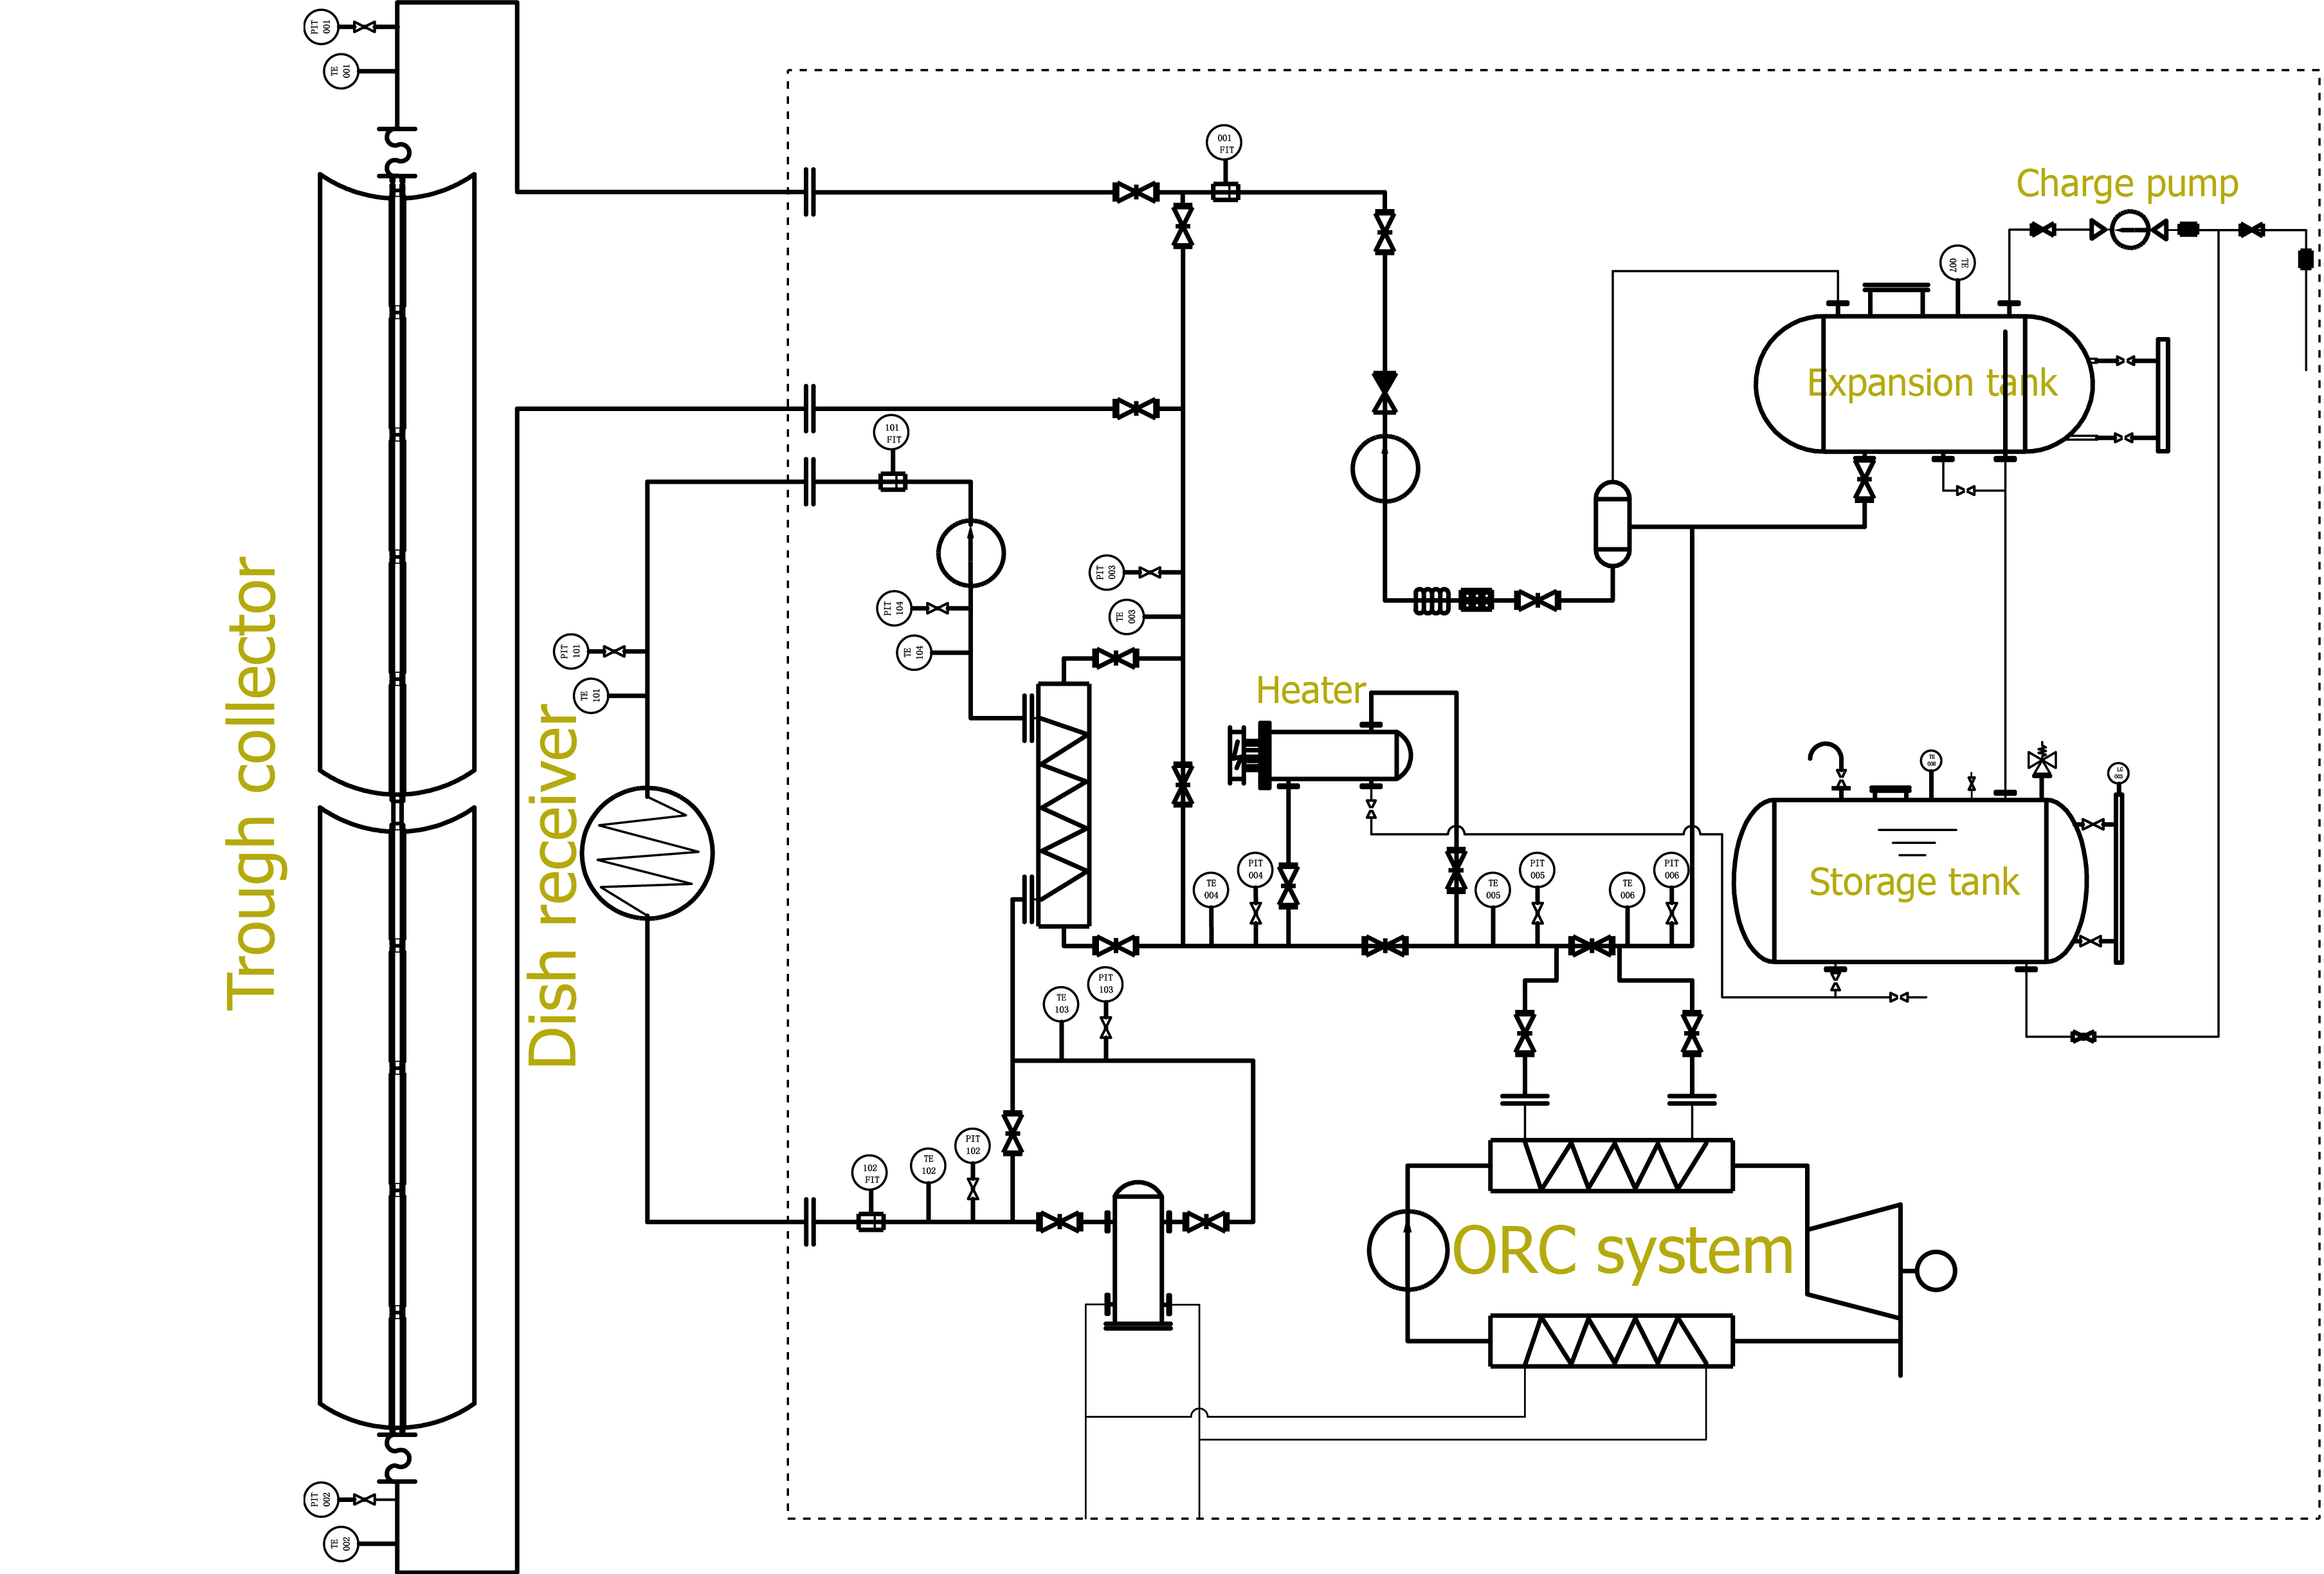
\includegraphics[width=1.0\textwidth]{fig/platform.png}
\caption{Schematic structure of the platform}\label{fig:platform}
\end{figure}
Figure~\ref{fig:platform} shows the schematic structure of the solar thermal power platform. 
Three circuits, the air circuit, oil circuit and organic fluid circuit, are created by different fluids. In the air circuit, air in the environment is first compressed in the compressor, and warmed by a heater, 
then heated in dish receiver, then flows into the air-oil heat exchanger to provide heat for Rankine cycle and finally %through the air pump
back to the environment. 
In the oil circuit, the oil is first heated in the trough collector and then flows into the air-oil heat exchanger to obtain the heat provided by the air. The heated oil flows 
into the evaporator of the ORC system to provide heat for the ORC system, then through the pump back to the trough collector.
In the organic fluid circuit, the organic fluid first absorbs the heat provided by the oil in the evaporator, then flows into the ORC turbine for expansion. After expansion, the organic fluid flows into the regenerator to recover part of the overheating heat, then into the condenser, and back to the regenerator to reuse the rejected heat, then through the pump back to the evaporator.

The following describes the key components of the platform.

\subsection{Trough collector}
The trough collector is east-west oriented due to land constrains. It is made of parabolic reflector, receiver and bracket. Figure~\ref{fig:TroughCollector} shows the photo of the trough collector. The reflector is 20$\,\mathrm{m}$ long, and 2.55$\,\mathrm{m}$ wide. The receiver consists of a glass tube and a metal black pipe, vacuum is maintained between the two to reduce heat loss. 
The external diameter of the glass tube is 0.11$\,\mathrm{m}$, and the internal diameter is 0.106$\,\mathrm{m}$.
The external diameter of the metal tube is 0.038$\,\mathrm{m}$, and the internal diameter is 0.035$\,\mathrm{m}$.
The bracket is applied to support the reflector and receiver. Its structure is safe enough to resist common windy, stormy and snowy weather conditions. The mechanical structures for rotation, positioning and connection are simple and reliable, easy for mounting, dismounting and transportation, and convenient for operation and maintenance.
Single-axis tracking system is applied on the trough collector system. The program algorithm is used for real-time automatic tracking with small tracking error. Manual mode is also an optional choice. The buttons in the control cabinet make it convenient to adjust the collector to the desired direction. In addition, it provides automatic protection and manual operation protection in case of emergency.

SINOPEC L-QD350 synthetic thermal oil is applied as the HTF of the trough collector system. It typical physical parameters are provided from the seller.

\begin{figure}[!ht]
\centering
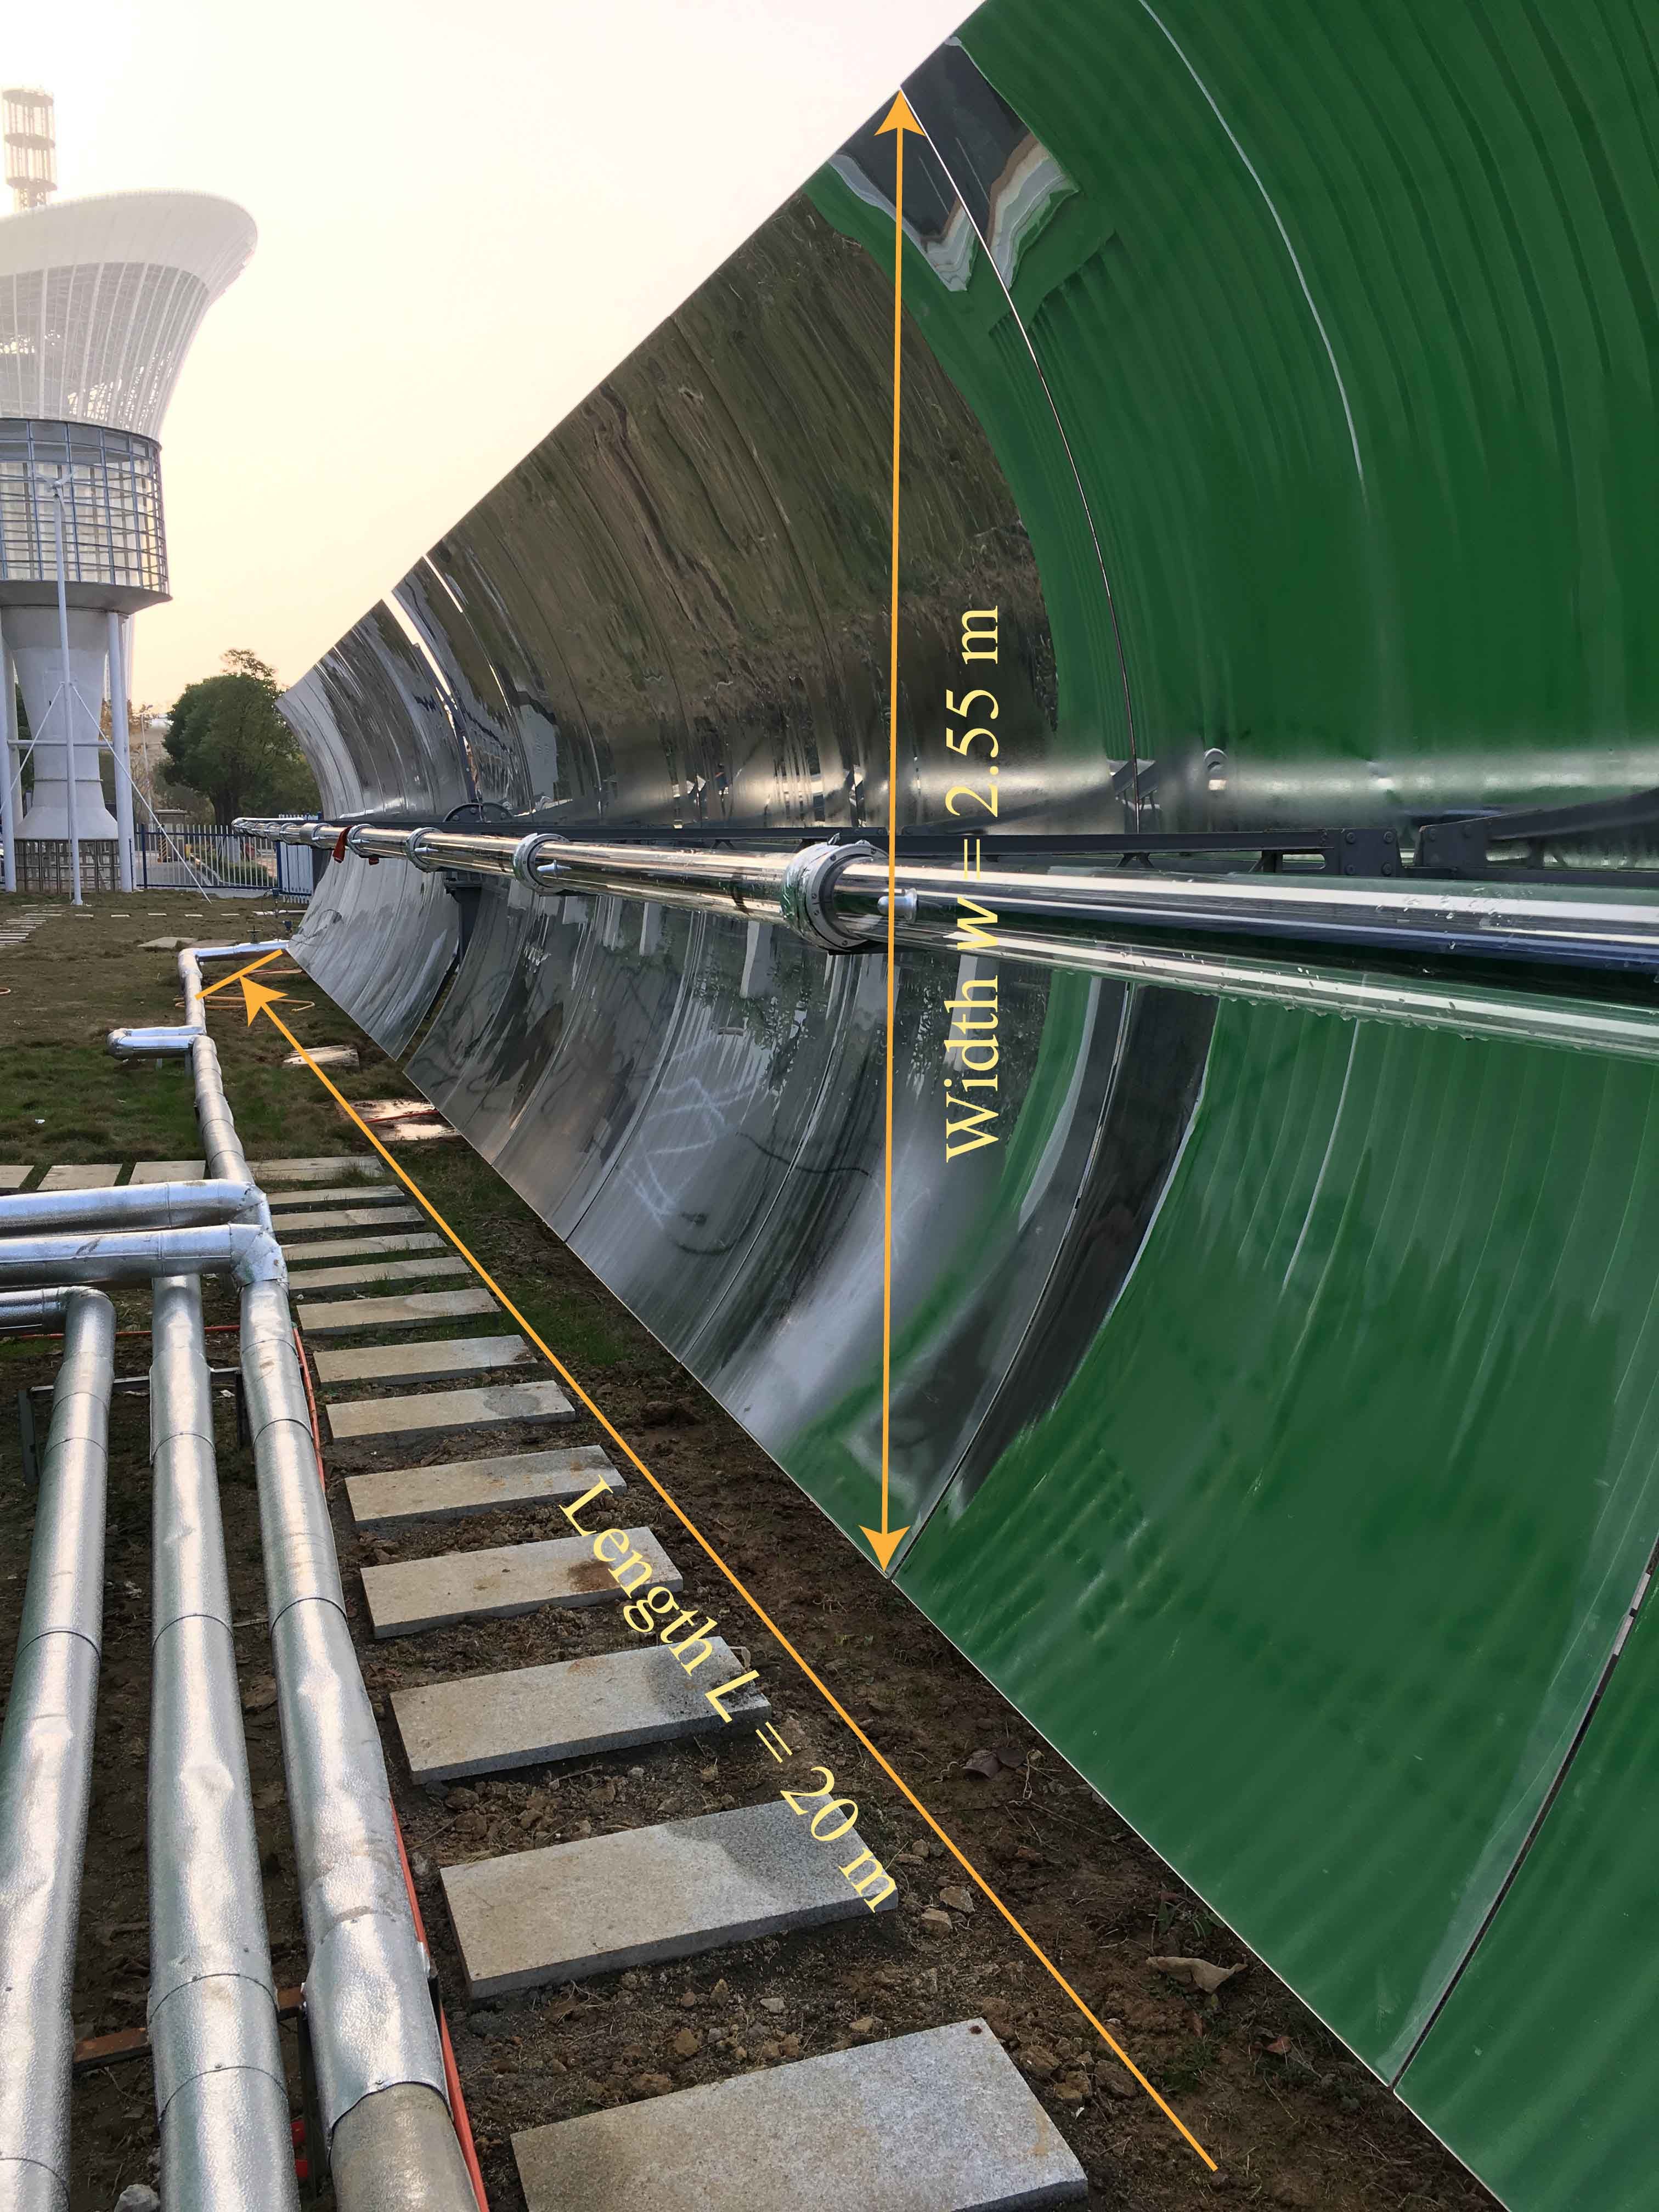
\includegraphics[width=0.7\textwidth]{fig/TroughCollector.jpg}
\caption{Trough collector of the platform}\label{fig:TroughCollector}
\end{figure}

\subsection{Dish collector}

\begin{figure}[!ht]
\centering
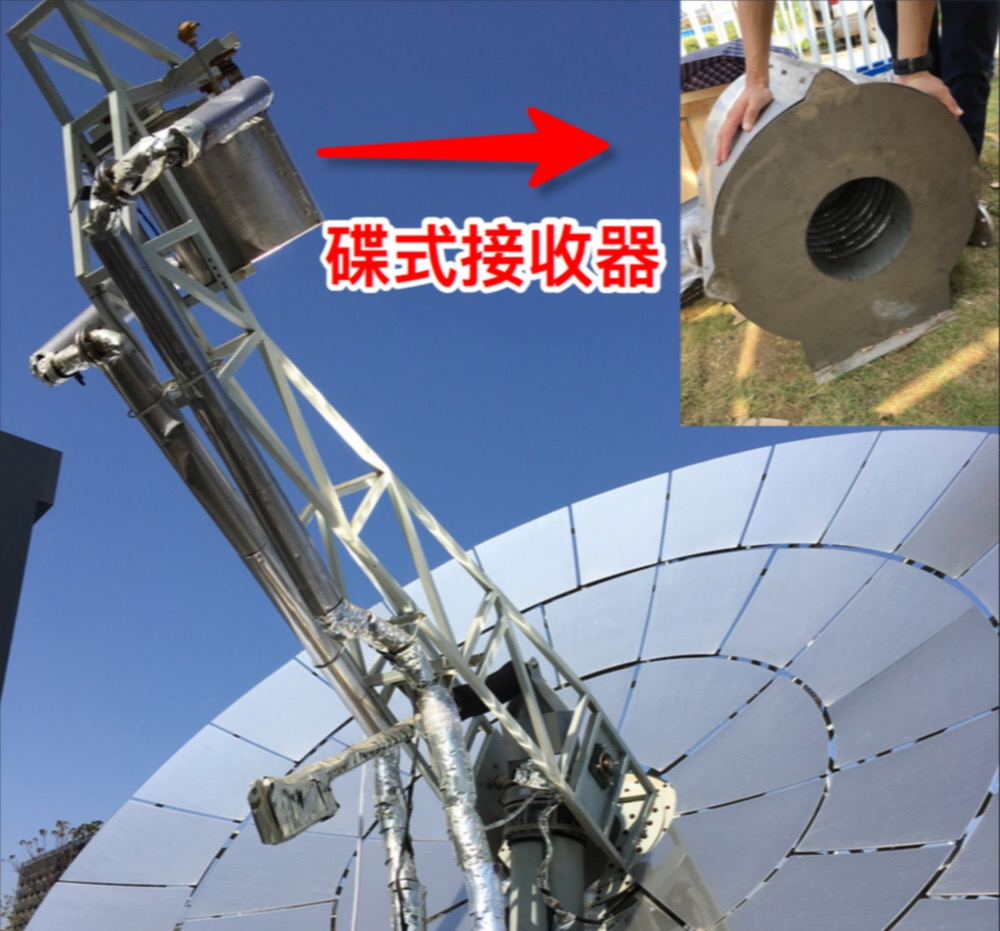
\includegraphics[width=0.7\textwidth]{fig/DishCollector.jpg}
\caption{Dish collector of the platform}\label{fig:DishCollector}
\end{figure}
Figure~\ref{fig:DishCollector} shows the photo of the dish collector. The reflector is made of multiple curved mirrors. When the aperture is facing to the sun, each of the mirrors reflects the sunlight to the focal point. 
%A notch was designed for rotating the collector. When calculating the effective area of the reflector
A self-designed receiver is mounted at the focal point of the dish reflector, as shown at top of the photo in Figure~\ref{fig:DishCollector}.
The key parameters of the dish collector are listed in Table~\ref{tab:ddc}. 
\begin{table}[htbp]
	\caption{Key parameters of the designed dish collector}
	\begin{center}
	\begin{tabular}{cccccc}
		\toprule
		Parameter		&	Value	&	Parameter		&	Value	&	Parameter		&	Value\\
		\midrule
		$d_{cav}$	&	0.45$\,\mathrm{m}$	&	$\epsilon_{insu}$	&	0.6	&	$\theta_{dc}$	&	20$^\circ$\\
		$\delta_{insu}$	&	0.11$\,\mathrm{m}$	&	$\alpha_{cav}$	&	0.87	&	$\gamma$	&	0.97\\
		$dep_{cav}$	&	0.45$\,\mathrm{m}$	&	$\delta_a$		&	0.002$\,\mathrm{m}$	&	$\eta_{shading}$	&	1\\
		$d_{ap}$	&	0.25$\,\mathrm{m}$	&	$d_{i,1}$	&	0.07$\,\mathrm{m}$	&	$\rho$	&	0.91\\
		$\lambda_{insu}$	&	0.06$\,\mathrm{W/(m\cdot K)}$	&	$A_{dc}$	&	23.3$\,\mathrm{m^2}$	&	\\		
		\bottomrule
	\end{tabular}
	\end{center}
	\label{tab:ddc}
\end{table}

The YYGN-GR-1A automatic two-axis tracking control system is used for the dish collector system. Both algorithm tracking method and sensor tracking method are applied for the tracking system. Usually, at the beginning of the focusing process, manual mode is applied to roughly rotate the collector towards the sun. Then switch to the automatic mode to precisely facing the sun. And the algorithm tracking method will take over and keep tracking the sun. This provides a more reliable tracking system with tracking error of less than 0.2$^o$ without cumulative error.
The control cabinet of the dish collector provides mechanical, electrical and other optional controls. It also monitors the wind speed and provides the function of set maximum wind speed for safety. When the wind is too strong, it will rotate the collector to a safe angle (facing the zenith).

\subsection{ORC system}
Hot oil (heated by the trough collector and/or the heater) is supplied to the ORC system. 
In the hot loop, input temperature of the supplied oil is 180$\,^\circ$C, and output temperature is 160$\,^\circ$C. Flow rate of 0.44$\,\mathrm{kg/s}$ is required to reach the nominal output gross power 1.5$\,\mathrm{kW}$. In the cold loop, input temperature of tap water is 30$\,^\circ$C, and output temperature is 37$\,^\circ$C. The water flow rate is about 0.83$\,\mathrm{kg/s}$.

\begin{figure}[!ht]
\centering
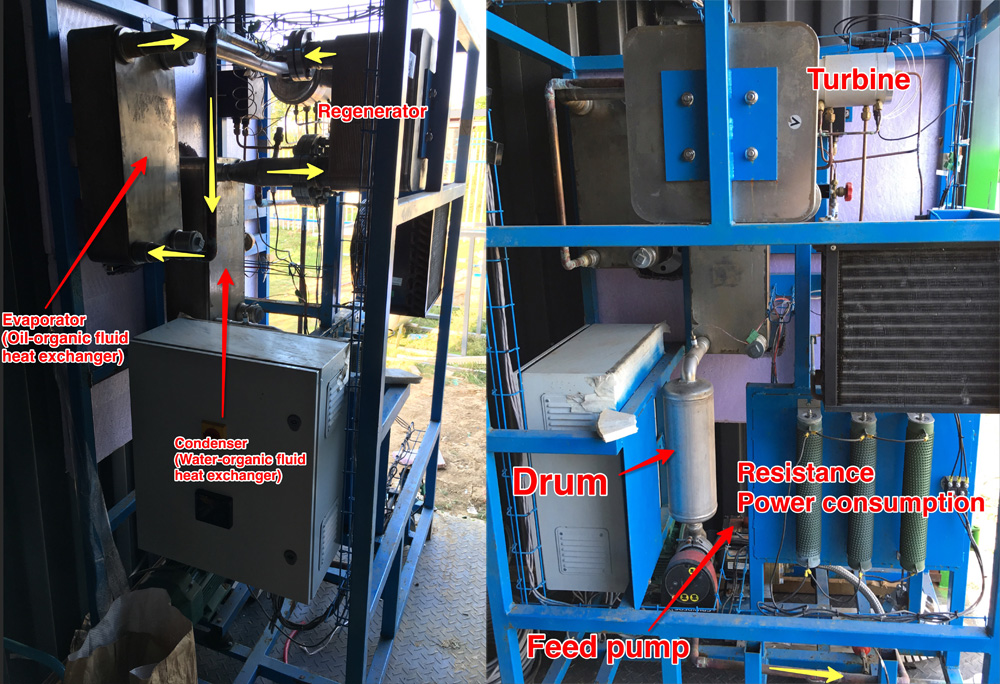
\includegraphics[width=0.7\textwidth]{fig/ORCsystem.jpg}
\caption{ORC system of the platform}\label{fig:ORCsystem}
\end{figure}
Figure~\ref{fig:ORCsystem} shows photos of the ORC system. It is made of evaporator, high speed ORC turbine, generator, regenerator, condenser, organic working medium pump, electrical control cabinet and the connection pipes.

The control cabinet provide a touch screen to control the ORC system. Both automatic mode and manual mode are provided. In the automatic mode, all the start up work and shut down work will be completed by procedure automatically. In the manual mode, detail parameters, such as organic fluid pump speed, much be set by hand, which provides precise control of the system.

\begin{figure}[!ht]
\centering
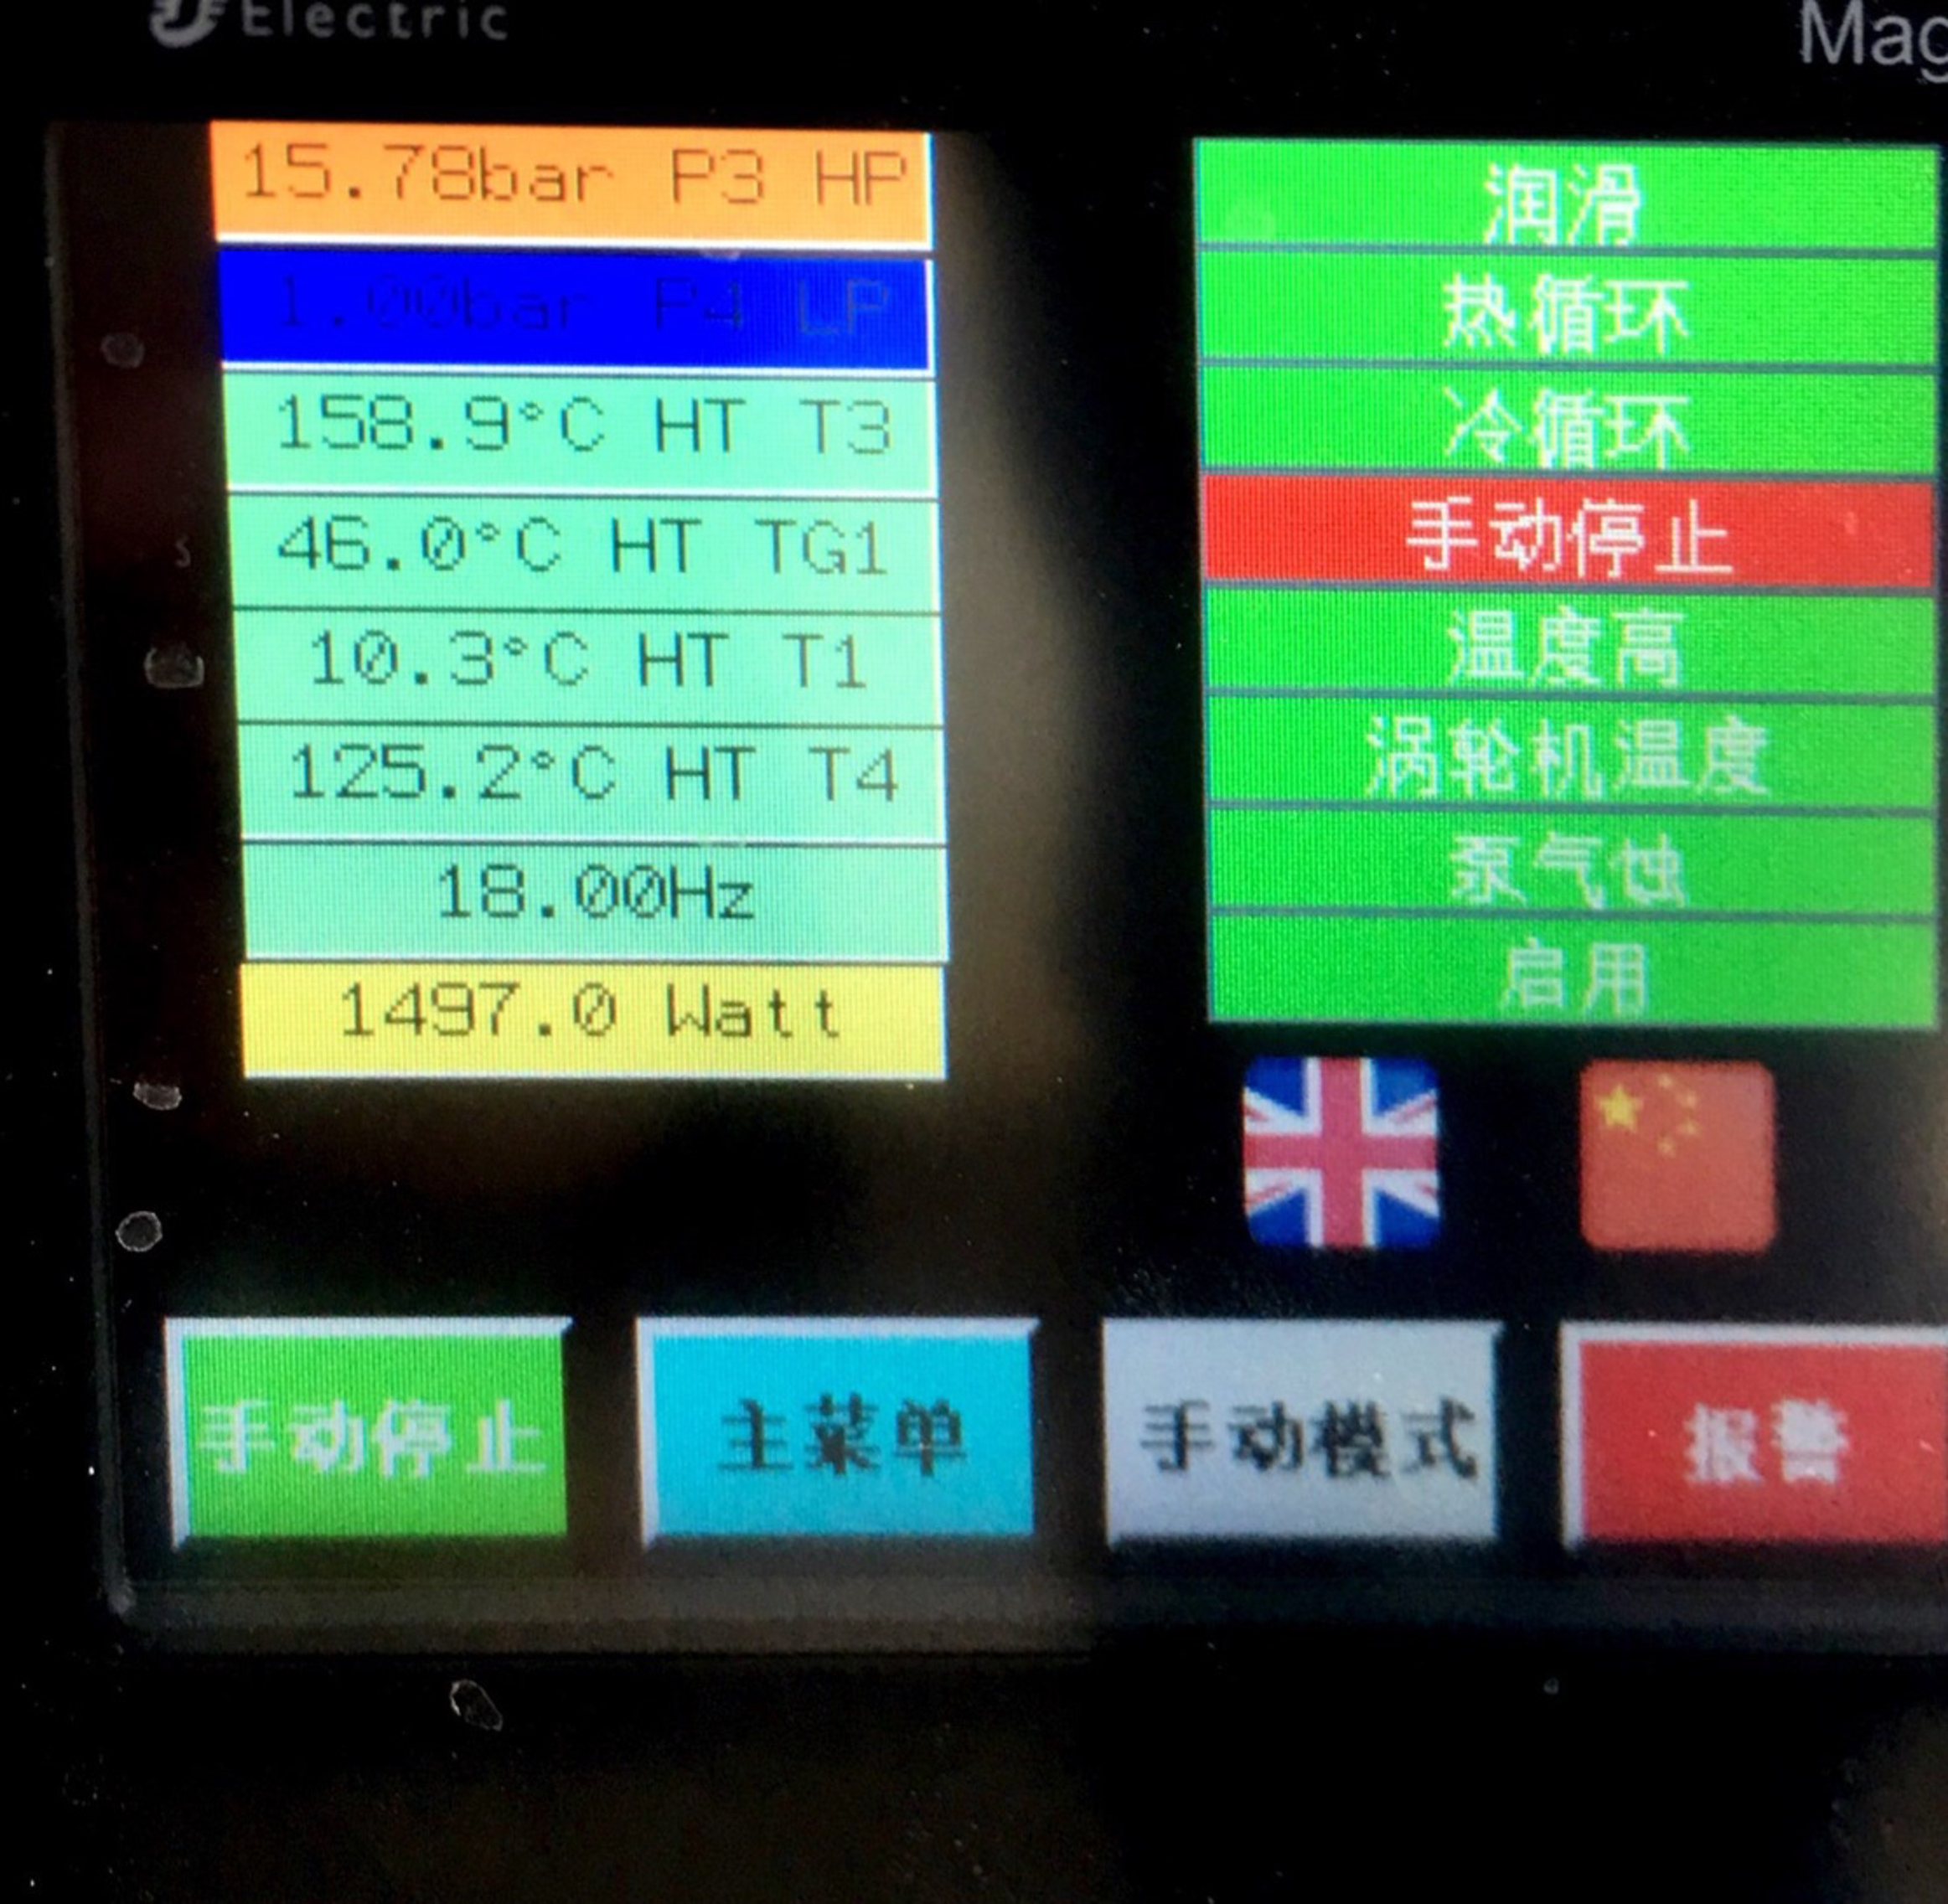
\includegraphics[width=0.4\textwidth]{fig/ControlCabinet}
\caption{Control screen of the ORC system}\label{fig:ControlCabinet}
\end{figure}

\subsection{Piping system}

Piping system provides the basis for fluid flow and heat exchange. Plus, it provides thermal insulation for hot fluids. Meters, pumps, valves, tanks and heaters are arranged in the piping system to maintain the normal and orderly operation.

Two heaters are used in the platform to increase the temperatures of the fluids (air and oil) to reach the experiment requirements when the solar irradiance is not enough. The two heaters have temperature sensors to keep the 
outlet fluid temperatures as required by changing powers.
 

%\subsection{Data collection system}

\section{Experiments}

In order to test the performance of the platform and validate the proposed models, relevant experiments were carried out.
\subsection{Trough collector experiment}

\subsection{Dish collector experiment}

\subsubsection{ORC system experiment}

\section{Result analysis}
\section{Platform evaluation}